\documentclass[border=3pt]{standalone}
% Preâmbulo compartilhado pelos diagramas TikZ da aula 11 (Localização por Grade e Monte Carlo)
\usepackage[T1]{fontenc}
\usepackage[utf8]{inputenc}
\usepackage{lmodern}
\usepackage{amsmath}
\usepackage{xcolor}
\usepackage{tikz}
\usetikzlibrary{arrows.meta,angles,quotes,decorations.pathmorphing,calc,
                positioning,shapes.geometric,shapes.misc,backgrounds,fit,
                math}

% Paleta (mesma dos SVGs originais)
\definecolor{dblue}{HTML}{2A5B8C}
\definecolor{dorange}{HTML}{B3541E}
\definecolor{dgreen}{HTML}{4A7C59}
\definecolor{dred}{HTML}{9C4B4B}
\definecolor{dcream}{HTML}{F4F1EA}
\definecolor{dshade}{HTML}{DDD7C9}

% Função gaussiana (não normalizada por padrão de escala visual)
\pgfmathdeclarefunction{gauss}{3}{%
  \pgfmathparse{1/(#3*sqrt(2*pi))*exp(-((#1-#2)^2)/(2*#3^2))}%
}

% Estilos comuns (prefixo d... para não colidir com chaves internas do pgf)
\tikzset{
  >={Stealth[length=2mm]},
  dguide/.style={gray!55, dashed, line width=0.4pt},
  daxis/.style={gray!60, line width=0.7pt, ->},
  dbody/.style={fill=black!3, draw=black!80, line width=1pt},
  dacc/.style={draw=dblue, line width=1pt},
  dlbl/.style={black!55, font=\small},
  dsub/.style={black!45, font=\footnotesize},
  dstate/.style={circle, draw=black!80, fill=dcream, line width=1pt,
                 minimum size=17mm, font=\large, inner sep=1pt},
  dobs/.style={circle, draw=black!80, fill=dshade, line width=1pt,
               minimum size=14mm, font=\large, inner sep=1pt},
  dbox/.style={rounded corners=2pt, draw=black!80, fill=dcream, line width=1pt,
               align=center, inner sep=6pt},
  dop/.style={circle, draw=black!80, fill=white, line width=1pt,
              minimum size=6mm, inner sep=0pt, font=\small},
  dtrans/.style={->, dblue, line width=1pt},
  dmeas/.style={->, dorange, line width=1pt},
  dcurve/.style={line width=1pt, dblue},
  dcurveb/.style={line width=1.4pt, dorange},
}

\begin{document}
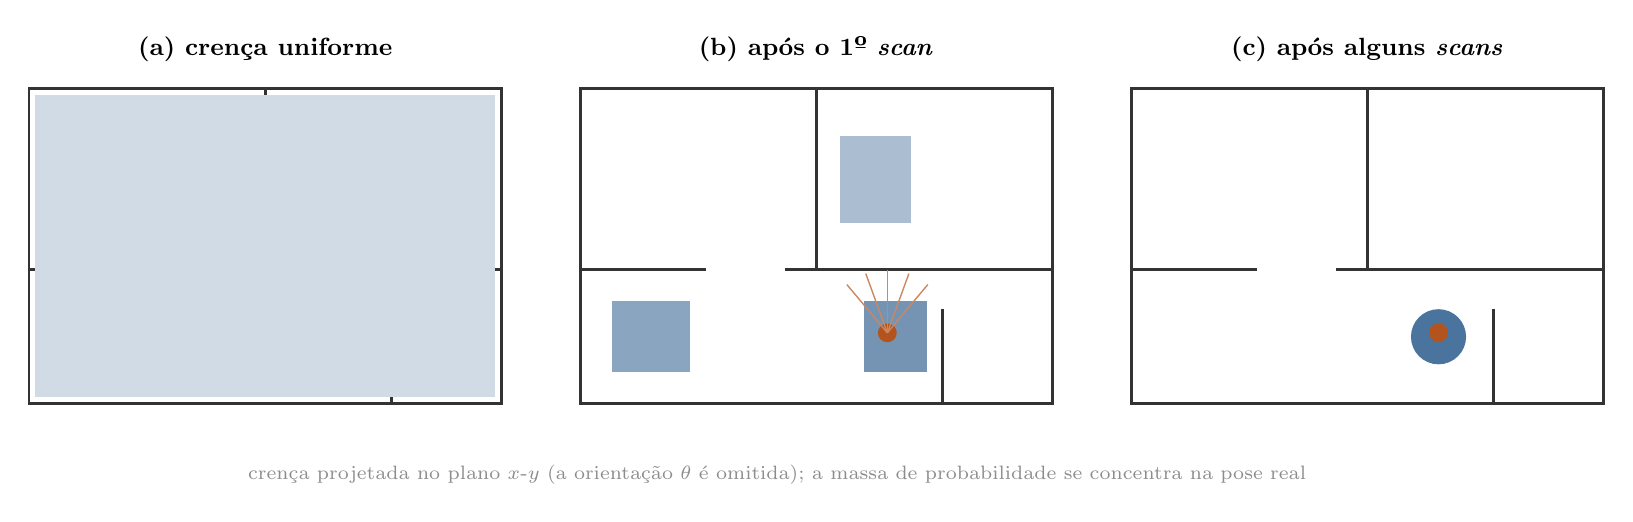
\begin{tikzpicture}[x=1cm,y=1cm,
   bel/.style={fill=dblue, draw=none}]
  \newcommand{\planta}{\draw[dbody, fill=white, line width=1pt] (0,0) rectangle (6,4); \draw[dbody, line width=1pt] (0,1.7) -- (1.6,1.7) (2.6,1.7) -- (6,1.7); \draw[dbody, line width=1pt] (3.0,1.7) -- (3.0,4); \draw[dbody, line width=1pt] (4.6,0) -- (4.6,1.2);}
  \begin{scope}
    \planta \fill[dblue!22] (0.08,0.08) rectangle (5.92,3.92);
    \node[font=\small\bfseries] at (3,4.5) {(a) crença uniforme};
  \end{scope}
  \begin{scope}[shift={(7,0)}]
    \planta
    \fill[dblue!55] (0.4,0.4) rectangle (1.4,1.3); \fill[dblue!65] (3.6,0.4) rectangle (4.4,1.3); \fill[dblue!40] (3.3,2.3) rectangle (4.2,3.4);
    \fill[dorange] (3.9,0.9) circle (0.12);
    \foreach \a in {-40,-20,0,20,40} { \draw[dorange!70, line width=0.5pt] (3.9,0.9) -- ++(\a+90:0.8); }
    \node[font=\small\bfseries] at (3,4.5) {(b) após o 1º \textit{scan}};
  \end{scope}
  \begin{scope}[shift={(14,0)}]
    \planta
    \fill[dblue!85] (3.9,0.85) circle (0.35);
    \fill[dorange] (3.9,0.9) circle (0.12);
    \node[font=\small\bfseries] at (3,4.5) {(c) após alguns \textit{scans}};
  \end{scope}
  \node[dsub, font=\scriptsize, align=center, text width=18cm] at (9.5,-0.9) {crença projetada no plano $x$-$y$ (a orientação $\theta$ é omitida); a massa de probabilidade se concentra na pose real};
\end{tikzpicture}
\end{document}
